\begin{figure}[H]
    \centering

    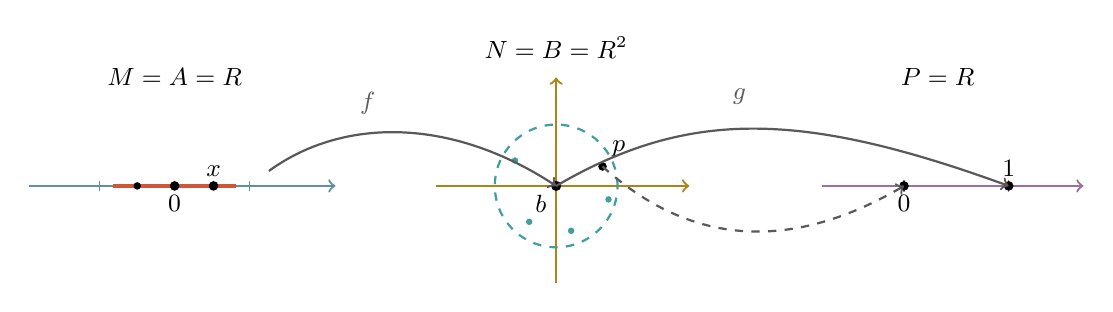
\begin{tikzpicture}[
        scale=0.95,
        every node/.style={font=\small},
        mline/.style={->, thick, SkyBlue!70!black},
        naxis/.style={->, thick, Goldenrod!80!black},
        pline/.style={->, thick, Plum!70!black},
        map/.style={->, thick, black!65},
        altmap/.style={->, thick, dashed, black!65},
        margin/.style={thick, dashed}
    ]
        \begin{scope}
            \node at (0,1.45) {$M=A=\mathbb R$};
            \draw[mline] (-1.95,0) -- (2.15,0);
            \draw[RedOrange!82!black, very thick] (-0.82,0) -- (0.82,0);

            \foreach \t in {-1,0,1} {
                \draw[SkyBlue!70!black] (\t,0.07) -- (\t,-0.07);
            }

            \coordinate (zeroM) at (0,0);
            \coordinate (xM) at (0.52,0);
            \coordinate (mEdge) at (1.26,0.20);

            \filldraw[black] (zeroM) circle (1.6pt) node[below] {$0$};
            \filldraw[black] (xM) circle (1.6pt) node[above] {$x$};
            \filldraw[black] (-0.50,0) circle (1.2pt);
        \end{scope}

        \begin{scope}[xshift=5.10cm]
            \node at (0,1.85) {$N=B=\mathbb R^2$};
            \draw[naxis] (-1.60,0) -- (1.78,0);
            \draw[naxis] (0,-1.30) -- (0,1.45);

            \coordinate (b) at (0,0);
            \coordinate (pN) at (0.62,0.26);
            \coordinate (nEdge) at (-1.52,0.30);
            \coordinate (nRight) at (1.55,0.30);

            \draw[margin, TealBlue!80!black] (b) circle (0.82);
            \filldraw[black] (b) circle (1.7pt) node[below left] {$b$};
            \filldraw[black] (pN) circle (1.4pt) node[above right] {$p$};

            \foreach \p in {(-0.55,0.34),(-0.36,-0.48),(0.20,-0.60),(0.70,-0.18)} {
                \filldraw[TealBlue!80!black] \p circle (1pt);
            }
        \end{scope}

        \begin{scope}[xshift=10.20cm]
            \node at (0,1.45) {$P=\mathbb R$};
            \draw[pline] (-1.55,0) -- (1.95,0);

            \coordinate (zeroP) at (-0.45,0);
            \coordinate (oneP) at (0.95,0);
            \coordinate (pEdge) at (-1.34,0.25);

            \foreach \q/\labelpos/\label in {zeroP/below/{$0$},oneP/above/{$1$}} {
                \draw[Plum!70!black] (\q) ++(0,0.08) -- ++(0,-0.16);
                \filldraw[black] (\q) circle (1.6pt) node[\labelpos] {\label};
            }
        \end{scope}

        \draw[map] (mEdge) .. controls (2.25,0.92) and (3.70,0.92) .. (b);
        \node[black!65] at (2.58,1.10) {$f$};

        \draw[map] (b) .. controls (6.85,1.02) and (8.35,1.02) .. (oneP);
        \node[black!65] at (7.55,1.20) {$g$};

        \draw[altmap] (pN) .. controls (6.95,-0.85) and (8.30,-0.85) .. (zeroP);
    \end{tikzpicture}

    \caption{Ilustração do Exemplo~\ref{ex:composicaoLimitesFalsa}.}
    \label{fig:composicaoLimitesFalsa}
\end{figure}
